
\rhead{\itshape Modélisation de la nouvelle approche}

\chapter{Modélisation de la nouvelle approche}

\section{Introduction}
L’internet des objets étend la technologie Internet actuelle en connectant différents types d'objets (objets ou appareils) entre eux et leur permet de communiquer intelligemment. ce concept est conçu pour connecter des millions d’objets, mais les objets avec ce nombre nécessitent de grands espaces de stockage et génèrent un trafic important, ce qui pourrait créer de nombreux problèmes au réseau. De plus, bien que les objets soient connectées les uns aux autres, ils ne sont pas nécessairement capable de communiquer entre eux. Leur capacité à communiquer entre eux dépend de la similitude du service auquel ils sont affectés. Ces lacunes sont dues au fait que les objets ne peuvent pas raisonner dans leur environnement et prendre ensuite des décisions et des actions intelligentes pour atteindre leurs objectifs.

Bien que l'ensemble du système connecté de l’loT manifeste la capacité de prendre des décisions et d'interagir intelligemment entre les objets, il le fait sur la base des règles implicites sans prendre en considération des modifications involontaires de l'environnement.


Tout le système peut quelque peu être représenté comme un système intelligent mais pas les objets. Ce sont les enjeux majeurs de l’loT en plus des enjeux de sécurité, de gouvernance et de normalisation. Nous rapplons queles lacunes de l'internet des objets sont le suivant: 

\begin{itemize}
    \item L’objet comme une seule entité dans l’loT n'est pas intelligent, mais tout le système est quelque peu intelligent.
    \item La prise de décision et les actions ultérieures dépendent du service.
    \item Les objets de l’loT sont connectés les uns aux autres, mais ils ne sont pas nécessairement capables de communiquer entre eux.
    \item Les objets ne peuvent communiquer avec d'autres objets que lorsqu'elles sont conçues pour exécuter les mêmes services système.
    \item L’loT souffre d'autres problèmes concernant la sécurité, la gouvernance et la normalisation.

\end{itemize}

La vision du concept loT est d'établir un système à grande échelle en connectant tout à l'Internet et en les faisant communiquer entre eux de machine à machine (M2M), L' loT tente d'aider les humains à décider de meilleures solutions de gestion des données pour leurs problèmes spécifiques au domaine en traitant les informations pertinentes à partir des objets interconnectées. Cependant, en raison des lacunes ci-dessus qui empêchent cette vision de devenir une réalité, nous proposons une nouvelle approche basée sur des agents logiciels pour atténuer les problèmes de l’absence de raisonnement et d'intelligence dans les objets des systèmes loT, En ayant de telles fonctions améliorées, notre nouvelle approche tente d'augmenter l'loT en incorporant des agents logiciels intelligents dans les objets pour améliorer les services qui pourraient être dérivés des interactions des agents logiciels dans ces objets.


\section{Architecture générale du système}

 Dans le domaine de l'IoT, les dispositifs dits IoT fournissent normalement de telles capacités de calcul et sont appelés edge nœuds, edge périphériques ou périphériques intelligents; même si, selon la granularité du scénario particulier, les périphériques peuvent avoir une capacité de calcul plus ou moins élevée. Le fait d'avoir une capacités de calcul dans le périphérique lui-même offre plusieurs avantages: le premier est que nous pouvons prétraiter les données obtenues dans l'edge périphérique et communiquer ces informations aux périphériques externes uniquement lorsque cela est pertinent ou nécessaire, économisant de nombreuses ressources du périphérique et améliorant la latence; le second est que l'appareil peut prendre sa propre décision, s'il est programmé pour lui, particulièrement utile lorsqu'il n'y a pas de connexion réseau.
 
Dans cette section, nous allons présenter l’architecture générale "IoT approach using multi-agent system for ambient intelligence" \cite{zouai2017iot} proposée de notre système. En effet, le système proposée est basé sur un système multi-agents (situé et mobile), en gardant l’avantage offert par ce paradigme et afin de maintenir le problème de communication entre les objets (IoT). Nous avons doté les objets de notre système avec des agents intelligents pour améliorer les services qui pourraient être dérivés des interactions des agents logiciels dans ces objets.

L’architecture générale de notre système  est une architecture collaborative pour l'IoT, qui est composée de plusieurs edge et fog nœuds et de cloud qui collaborent dans un écosystème orienté services et agents tout au long de la coopération des agents logiciels et du CEP.


Nous avons trois couches dans l'architecture, ces couches se concentreront conceptuellement sur la détection, la passerelle et la couche de service et seront matérialisées dans les edges nœuds, de fog et de cloud correspondants. La figure  \ref{fc7}  montre une architecture illustrative dans laquelle un nœud de cloud, deux  fog nœuds et cinq edge nœuds ont été inclus. Cependant, l'architecture pourrait avoir des nœuds supplémentaires de tous les types (certains fog et edge nœuds supplémentaires sont également représentés en petit). Dans tous les cas, on s'attend à ce que l'architecture ait plus de edge nœuds  que de fog nœuds et donc plus d’edge nœuds que de cloud nœuds.
\subsection{Description des couches et des composants}

Comme mentionné précédemment, dans notre architecture, nous avons des edge nœuds, fog nœuds et des nœuds de cloud, comme expliqué dans les paragraphes suivants.

\begin{figure}[H]
\centering
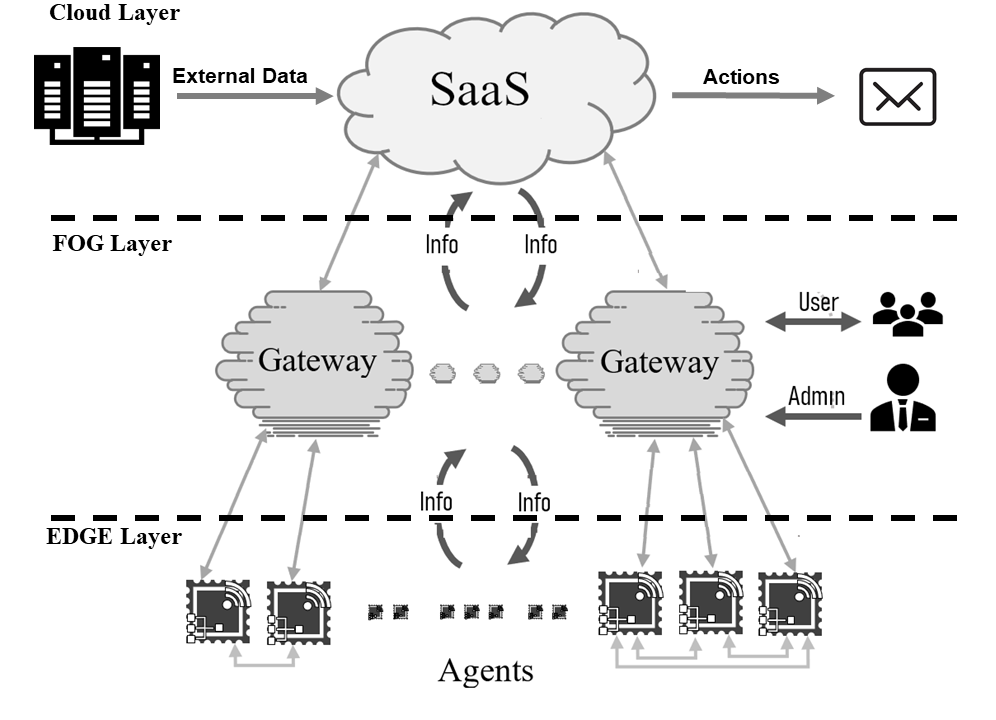
\includegraphics[scale=0.5]{chap1/ARCH_G.png}
\caption{Architecture  en couches du système.}
\label{fc7}
\end{figure}

\subsubsection{Edge nodes} Il faut se rappeler que les IoT devices, représentés comme des edge nœuds, ont généralement des ressources de calcul limitées, c'est pourquoi (1) les logiciels qu'ils incorporent doivent consommer peu de ressources en exécution et (2) les communications via Internet doivent être autant limitées que possible pour économiser les ressources. Avec cet objectif, nous avons déployé un agent logiciel dans chaque edge nœud, car les agents consomment peu de ressources et disposent d'une autonomie et d'une capacité d'intelligence et de décision suffisantes pour filtrer les informations réellement nécessaires à transmettre et celles qui ne seront utilisées qu'en interne dans le nœud. L'intelligence de l'agent est programmée à partir d'une série de règles de comportement; de cette manière, le comportement du dispositif pourra s'adapter à l'environnement prenant des décisions en fonction des informations obtenues de ses capteurs et des informations obtenues des autres edge nœuds connectés au réseau et du fog nœud. Les agents pourront communiquer entre eux et traiter et analyser les informations détectées et reçues des autres acteurs et prendre les décisions correspondantes sans avoir besoin de contacter l'utilisateur.


\subsubsection{Fog nodes}
Ce sont les appareils qui serviront de passerelles entre les appareils IoT en edge et (a) l'utilisateur et (b) les nœuds dans le cloud. D'une part, toutes les communications des agents logiciels avec l'utilisateur final se feront via un Broker dans la passerelle: les edge devices peuvent envoyer des messages à un topic dans le Broker auquel l'utilisateur est abonné. D'autre part, les communications entre l’edge et le cloud se feront également via le Broker de manière bidirectionnelle. Un tel Broker sera connecté à un moteur CEP dans l’edge nœud pour traiter les données reçues et détecter les informations pertinentes pour l'autre partie. Autrement dit, (1) le cloud envoie des informations au fog, le moteur CEP traite ces informations et si un modèle est satisfait, il soumet les informations pertinentes au edge; (2) l'edge envoie des informations au fog, le moteur CEP traite ces informations et si un modèle est respecté, il soumet les informations pertinentes au cloud. Bien sûr, un modèle peut être rencontré à partir des informations reçues à la fois de l’edge et du cloud. Les utilisateurs et le cloud auront différents topic auxquels s'abonner.

\subsubsection{Cloud Node}
Le nœud cloud a une communication bidirectionnelle avec les fog  nœuds. D'une part, le nœud cloud s'abonne aux topic de message des fog nœuds, ce qui lui permet d'obtenir des informations de tous ces nœuds et de prendre des décisions de plus haut niveau. Ces informations sont acquises avec d'autres sources de données hétérogènes et traitées via une SOA 2.0 compatible CEP. Le moteur CEP peut détecter des situations d'intérêt soit pour des tiers, soit pour des fog nœuds et les soumettre au Broker de messages correspondants auxquels ces acteurs pourraient s'abonner. Il est important de se rappeler qu'il pourrait y avoir plus de nœuds dans le cloud qui pourraient en même temps communiquer avec d'autres nœuds dans le cloud, mais pour plus de simplicité, nous n'allons en représenter qu'un.


Pour mettre en place le système, tout d'abord, les edges dispositifs  seront programmés avec les agents logiciels et les règles correspondantes avec les actions qu'ils peuvent effectuer en fonction des informations reçues des capteurs, des autres agents, de la passerelle et de l'utilisateur. Ces règles comprendront non seulement des actions telles que la mise en marche du climatiseur, mais également les informations susceptibles d'être diffusées aux agents restants ainsi que les informations à soumettre à l'utilisateur ou au Broker de la passerelle à traiter dans le moteur CEP. Deuxièmement, nous déploierons et configurerons le Broker  de messages et le moteur CEP dans le fog nœud, qui recevront les données de l’edge, d'autres fog nœuds et de cloud, comme expliqué précédemment. A cet effet, les acteurs seront abonnés aux topics  correspondants. De plus, nous déploierons les modèles conçus dans le moteur CEP. Enfin, nous déploierons également un Broker de messages et SOA 2.0, avec un moteur CEP intégré, dans le cloud. Nous nous abonnerons également au Broker  de messages aux sources de données d'intérêt, ainsi qu'aux fogs nœuds correspondant au scénario en question, et nous déploierons les patterns conçus. Nous déploierons également d'autres actions souhaitées lorsqu'un modèle est respecté (soumission de notification, offre de service, etc.).


\section{Architecture détaillée de système}
Dans cette section nous allons présenter les détails de notre conception.
\subsection{IoT Gateway}
Le dispositif IoT Gateway est un moyen de normaliser les informations provenant de l'environnement ambiant pour la perception des agents. Cet étalonnage est nécessaire en raison de l'hétérogénéité des protocoles des différents fabricants. Ainsi, le MAS (système multi-agent) perçoit l'environnement ambiant via la passerelle et agit sur celui-ci sans se soucier du format des données perçues. Cette geteway est composée de deux couches \cite{zouai2019ambiance}.


\textbf{Java Agent DEvelopment Framework:} JADE est un Framework de développement de systèmes multi-agents, open-source et basé sur le langage Java. Ce dernier assure une communication transparente par l’échange de messages dans le langage normalisé FIPA-ACL, la plateforme JADE  a été ajoutée pour faciliter la communication entre les agents;


\textbf{MQTT Broker:} Nous avons doté l'IoT  Gateway d'un MQTT Broker pour faciliter le processus de communication entre l'utilisateur et les objets tout en réduisant le trafic du réseau et d'économiser l'énergie du dispositif intermédiaire (IoT Gateway).
\begin{figure}[H]
\centering
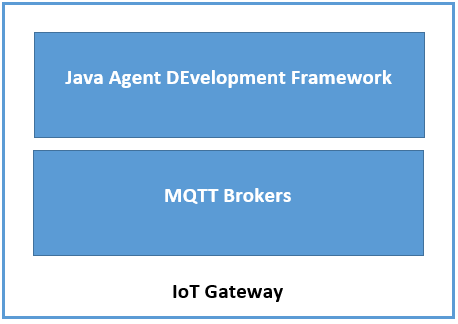
\includegraphics[scale=0.8]{chap1/fc8.png}
\caption{Architecture proposée IoT Gateway}
\label{fc8}
\end{figure}

\subsection{Agent de sécurité}
L’architecture de cet agent illustré dans la figure \ref{fc9} est composée de cinque éléments qui sont \cite{zouai2017iot} : 

\textbf{Environnement (Environment) :} il est constitué par l’environnement réel (maison, appartement, lieu de travail), il contient les composants de l’utilisateur et les composants voisins (l’autre composant situé au même endroit).


\textbf{Capteurs (Sensors):} c'est un appareil utilisé pour transformer le statut d'une grandeur physique observée (environnement) en une quantité utilisable (mesures). Tels qu'une tension électrique, une hauteur de mercure, une intensité ou la déviation d'une aiguille. Il y a souvent une confusion entre capteur et transducteur: un capteur est au moins composé d'un transducteur.


\textbf{Base historique des etats (Historical DB):} c'est un outil pour stocker l'historique d'informations fourni par les capteurs (l'état de l'environnement) et les états des autres composants du système.



\textbf{Base de règles (Rules DB):} elle rassemble la connaissance de l'agent. elle contient des règles pour aider l'agent à prendre des décisions. De telles décisions changent son état en fonction du état actuel de l'environnement et des états d'autres agents. La base de règles est mise à jour en fonction des nouveaux statuts et besoins de l'environnement. Les règles  représentent la connaissance générale de la sécurité et les constatations factuelles.


\begin{figure}
  
\centering
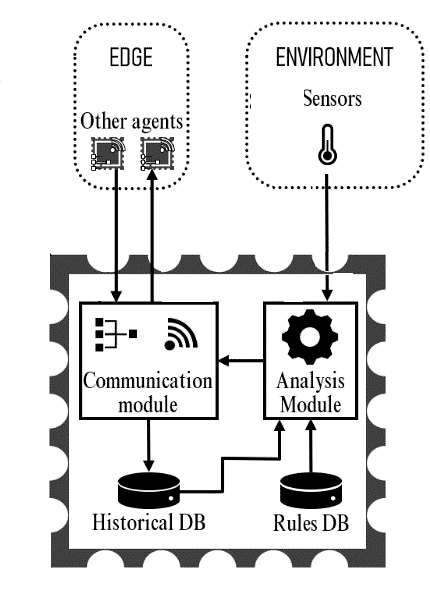
\includegraphics[scale=1.2]{chap1/agent2.png}
\caption{Architecture concrète de l'agent de sécurité}
\label{fc9}
\end{figure}
\subsubsection{Diagramme d'état}
Le diagramme d'état de la figure \ref{fc10} représente les états de la sécurité de l'agent et les conditions permettant de passer d'un état à d’un autre. L'enchainement entre les differents états et décrit de la maniére suivante: 


 L'agent commence à percevoir  l'environnement et attend les messages des autres agents. S'il y a un message, l'agent passe à l'état d'analyse des informations. Il compare les règles de sécurité avec les informations fournies par les agents et les données de détection. S'il existe une règle vraie (la règle est réalisable), l'agent envoie des ordres aux autres agents afin de contrôler le problème. L'agent informe l'utilisateur et le service qui peut gérer cette situation.



\begin{figure}[H]
\centering
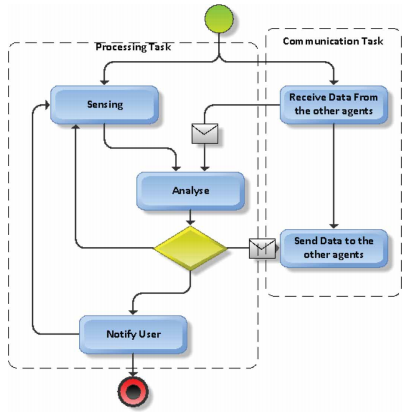
\includegraphics[scale=0.8]{chap1/fc10.png}
\caption{Diagramme d'état de l'agent de sécurité}
\label{fc10}
\end{figure}
\subsection{Dispositif IoT}
Comme expliqué précédemment, l'architecture IoT actuelle est trop rigide (voir Figure \ref{fig1} dans le chapitre 1) et ses objets ne sont pas autonomes. De plus, il n'est pas cognitif pour la construction de dispositifs IoT intelligents et autonomes.


Pour le dispositif IoT, nous avons proposé une extension  "Ambiance Intelligence Approach Using IoT and Multi-Agent System" \cite{zouai2019ambiance} en quatre couches. En particulier, nous avons ajouté une couche d'agent dans l'architecture, telle que présentée dans la figure \ref{fc11}. Nous avons intégré cette couche pour garantir les caractéristiques d'autonomie et d'intelligence de l'architecture IoT de cette manière, les objets conservent les caractéristiques d'autonomie et d'intelligence de l'agent.


Comme on peut le voir à la figure \ref{fc11}, nous avons inclus la couche d'agent entre la couche application et la couche réseau. La raison en est que l'agent proposé est un logiciel et qu'il doit utiliser la couche Network and Data Communication (NDC) pour: échanger des informations avec les appareils se trouvant à proximité; les informations reçues d'autres dispositifs et les informations captées par les capteurs sont les données sur lesquelles l'agent base ses décisions. L'agent utilise la couche physique (couche réseau et couche de perception ) en tant que capteurs pour détecter l'environnement et traiter ces informations réelles. De cette façon, le comportement de l'agent change en fonction de ces informations. En conséquence, cela modifie un ensemble de décisions utilisées dans la couche logicielle en fonction du but qui lui est destiné.


Le dispositif  IoT c'est l'élément central de cette section. Nous y avons ajouté la couche d'agent afin de doter le périphérique d'une sorte d'auto-intelligence, De cette manière, l'appareil est capable d'adapter et de mettre à jour le statut de l'environnement, grâce aux informations obtenues par les capteurs. L'agent traite et analyse ces informations. En conséquence, il prend la décision appropriée sans contacter l'utilisateur \cite{zouai2019ambiance};
\begin{figure}[H]
\centering
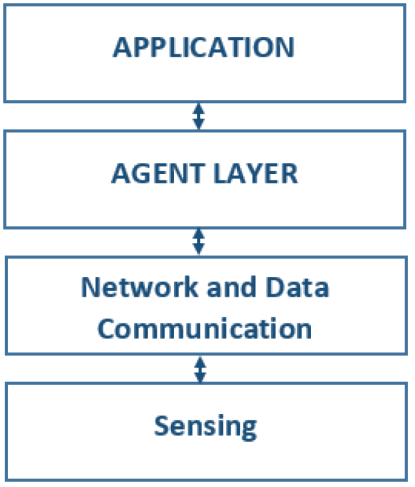
\includegraphics[scale=0.6]{chap1/fc11.png}
\caption{Architecture IoT Device}
\label{fc11}
\end{figure}
\subsection{Agent de santé}
L'agent de santé est intégré dans un composant physique, il peut contrôler l'état de santé de l'utilisateur de manière autonome et continue à travers les informations fournies par son smartphone, fit-bit montre, les autres agents...


Le smartphone fournit des informations telles que le nombre de pas que l'utilisateur fait, sa vitesse, les endroits qu'il a visités et les chemins qu'il a empruntés. En programmant l'alarme, le pourcentage d'éclairage et l'utilisation de l'appareil, nous pouvons connaître l'heure de sommeil de l'utilisateur, l'heure de réveil et la durée du sommeil, Nous pouvons confirmer ces informations à travers les informations que nous recevons d'autres agents telles que le temps d'éteindre l'éclairage et le mouvement de l'utilisateur à la maison, qui sont des informations importantes pour connaître la nature de sa santé.


Grâce à la liste d'achats qui nous est fournie en utilisant une carte de crédit, nous pouvons connaître la qualité et la nature des aliments qu'il mange.


Grâce à la communication de l'utilisateur avec les autres à travers les médias sociaux, par téléphone, à la maison et à travers l'histoire de la recherche sur Internet, nous pouvons extraire son état psychologique à travers l'analyse des informations précédentes et le développement de ses vélos vocaux pendant la conversation.
L'agent analyse toutes les informations précédentes et à travers lui il peut extraire la situation approximative de la santé de l'utilisateur, l'agent fournit des conseils sur une base régulière et continue à l'utilisateur afin de maintenir sa santé.
\begin{figure}[H]
\centering
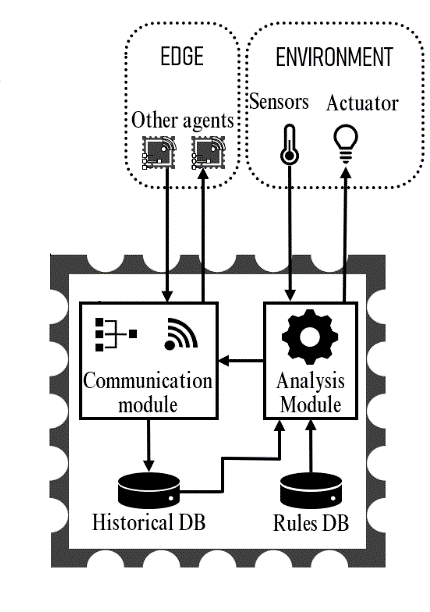
\includegraphics[scale=1.5]{chap1/agent.png}
\caption{Architecture concrète de l'agent «Health Care»}
\label{fc12}
\end{figure}

\begin{itemize}
    \item \textbf{ Environnement:} qui est perçu et contrôlé par l'agent de soins de santé qui est l'utilisateur du système. L'ensemble des perceptions est l'état actuel de la santé et des informations physiques.
    \item \textbf{Historique des états:} c'est une base de données qui contient d'anciennes informations sur la santé de l'utilisateur. Ses informations sont utilisées pour prédire ce qui se passerait et soyez prudent avant de tomber dans un état critique.
    \item \textbf{Base de Règles:} est composée d'un ensemble de règles qui représentent des observations factuelles et  des connaissances générales sur le domaine médical.
    \item \textbf{Module d'action:} permet aux agents de santé de mener un raisonnement logique et de tirer des conclusions à partir l'historique des états  et d'une base de règles.
\end{itemize}
\subsection{La modélisation de l'IoT Robot}
L'Internet des objets\cite{29}\cite{30} est un réseau d'objets principalement supportés par des dispositifs électroniques et des composants électroniques tels que des capteurs et des cartes électroniques. Ces objets peuvent être des périphériques physiques et virtuels, des capteurs ou des actionneurs. L'environnement intelligent nécessite beaucoup de capteurs et à différents endroits. Le coût de ces capteurs est cher. Pour réduire le coût de ces capteurs, nous avons proposé un robot mobile comportant une gamme de capteurs différents qui vont détecter l'environnement et envoyer des informations et des données aux objets de

l'environnement\cite{31}\cite{15}. À l'aide de ce robot, On n'aura pas besoin de mettre de capteurs partout puisque le Robot qui doté de capteurs se deplace aux endroits désirés. La  communication entre le robot et les objets IoT dans l'environnement se fait via le protocole MQTT\cite{32} .


Les objets IoT peuvent contrôler le robot directement via les commandes reçues par le robot. 

Nous avons implémenté ce robot avec une carte électronique perfectionnée Raspberry Pi B dotée de deux capteurs et d’une carte Arduino UNO pour la gestion des mouvements de robot \cite{zouai2019new}. Il est également équipé de capteurs pour empêcher le robot d'entrer en collision avec des barrières et des obstacles. Ces capteurs aident également le robot à surmonter les obstacles de manière autonome et aident à tracer un contour partiel de l'environnement environnant lorsque le schéma est un cercle de 4 mètres de diamètre et la commande du robot effectuée via un smartphone. Les commandes envoyées via le réseau local au robot si le smartphone et le robot sont connectés dans la même passerelle. Si le robot est distant, il reçoit les commandes via le réseau public Internet.


Nous avons fourni au robot une caméra orientable pour visualiser l'environnement. Il est contrôlé à distance par les commandes envoyées de l'exterieurs. Le serveur de caméra (Motion) envoie les images capturées à l'utilisateur en temps réel et directement. Motion est un système de surveillance assez complet. Il est extrêmement personnalisable: détection de mouvement, enregistrement image par image, enregistrement vidéo, laps de temps.


\subsubsection{Description de IoT Robot}
IoT Robot est composé principalement de 03 modules dont chacun contient des composants differents \cite{zouai2019new}.

\textbf{Le module de déplacement:} est le module responsable du mouvement du robot et de son déplacement. Ce module transforme l'énergie électrique en énergie cinétique à travers les moteurs du robot.

\textbf{Le module de détection:} est le module responsable de la détection du support externe. Cette unité convertit les valeurs physiques de l'environnement en valeurs numériques pouvant être stockées et analysées. Ce module relie le monde réel au monde numérique.


\textbf{Le module de communication :} est le module responsable de l’interaction du robot avec l’utilisateur en recevant des commandes, des rapports et des images sur l’environnement.




\begin{figure}[H]
\centering
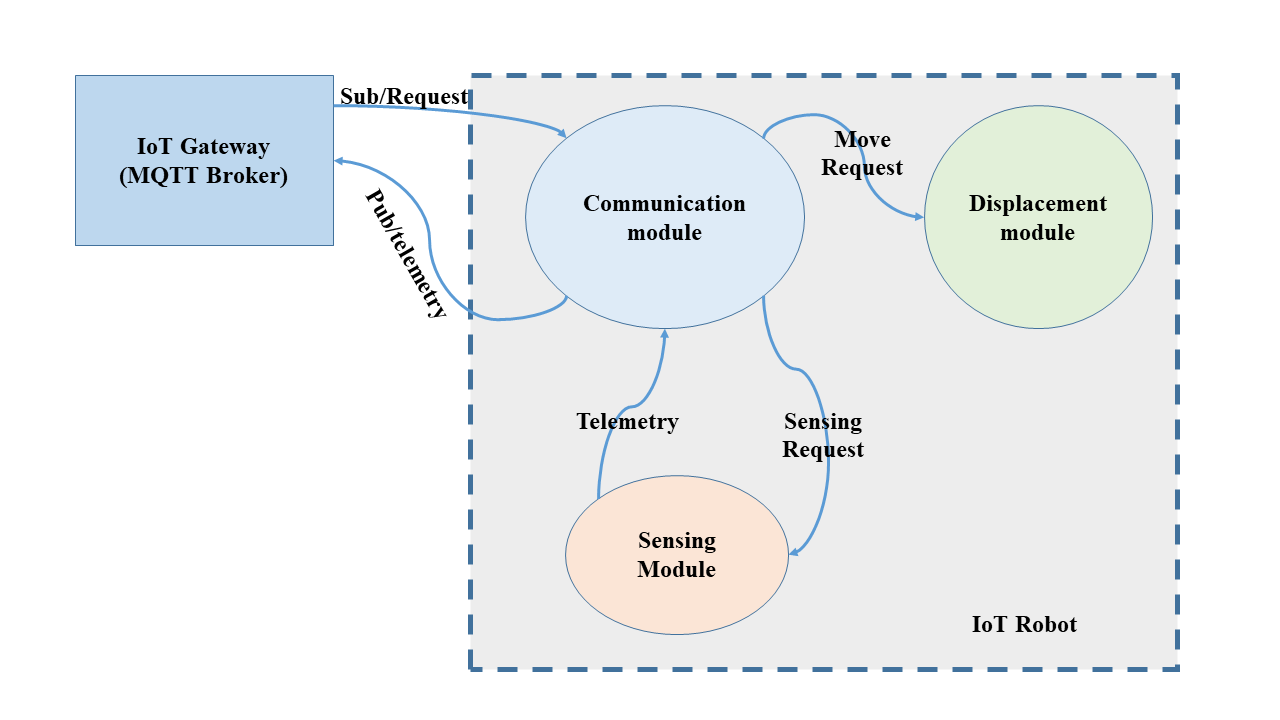
\includegraphics[scale=0.35]{chap1/Presentation23.png}
\caption{Modules d'IoT Robot}
\label{fc13}
\end{figure}

\subsubsection{Diagramme d'état}
Ce diagramme montre comment les pièces du robot interagissent les unes avec les autres pour atteindre leurs objectifs de manière idéale.

\begin{itemize}
    \item Le module de communication reçoit des commandes de l'utilisateur, ces éléments doivent être l'état initial.
    \item Le module de communication dirigera la commande en fonction de son type. S'il s'agit d'un ordre de commande de déplacement ou de détection.
    \item S'il s'agit d'un mouvement, le module de déplacement l'exécutera directement. 
    \item Le module de détection détecte l'environnement à travers les capteurs, prend des photos de l'environnement et les envoie directement et en temps réel à l'utilisateur.
\end{itemize}
\begin{figure}[H]
\centering
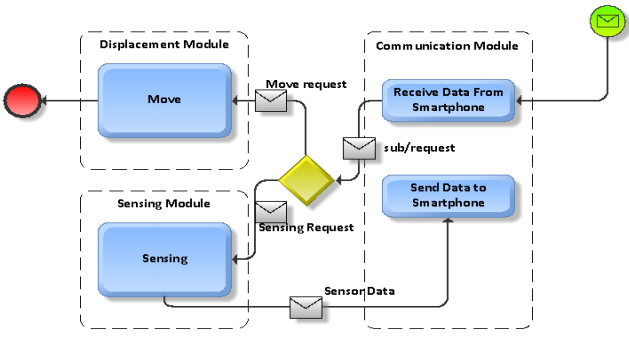
\includegraphics[scale=0.8]{chap1/fc14.png}
\caption{Diagramme d'état de IoT Robot}
\label{fc14}
\end{figure}
\subsection{Simulateur de maison intelligente}
Une maison intelligente consiste à connecter les différents appareils et systèmes de la maison afin qu'ils puissent être contrôlés de n'importe où et provoquer l'interaction souhaitée entre eux. Ces appareils sont des objets connectés via un réseau qui a une fenêtre sur Internet. Ce réseau d'objets s'appelle l'Internet des objets (IoT). L'IoT peut s'appliquer à plusieurs domaines: les villes intelligentes (villes totalement ou partiellement connectées à Internet leur permettant d'optimiser leurs capacités comme la gestion du trafic et le traitement de l'eau), la santé, les wearables (toutes les technologies portables telles que les montres connectées et les localisateurs), transport, mais aussi les lieux de travail, la production et les maisons \cite{zouai2017smart}.
\subsubsection{Conception de l'API Simulateur}
Notre simulateur est conçu en deux parties; une partie invisible à l'utilisateur (c'est-à-dire ne peut pas voir le contenu) contient les deux couches (API du simulateur, interface graphique du simulateur), et la deuxième partie visible à travers le code qui est classe publique.
\begin{figure}[H]
\centering
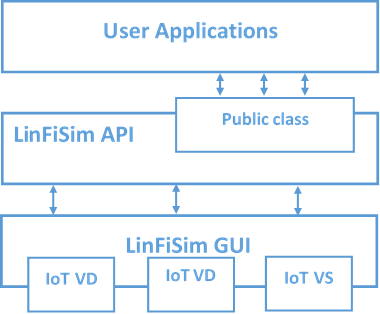
\includegraphics[scale=0.8]{chap1/fc15.png}
\caption{Architecture de l'API du simulateur}
\label{fc14}
\end{figure}

\paragraph{Composantes de l'API} Dans cette section, nous expliquons chaque composante de notre API, son contenu et son mode de fonctionnement.
\subparagraph{Interface utilisateur graphique (GUI) du simulateur:} l'interface utilisateur graphique (GUI) du simulateur est l'environnement graphique que l'utilisateur peut voir à l'écran et que l'interface contient.

\textbf{\textit{Périphérique virtuel IoT:}} le périphérique virtuel Internet des objets (IoT VD) est un objet virtuel qui simule un périphérique réel tel que (TV, climatiseur et lumière ...), chaque IoT VD a trois statuts possibles: {ON, OFF, SUSPENDU}, dans l'environnement du simulateur.

Pour tester notre API, Nous nous sommes concentrés sur les appareils les plus importants utile dans chaque maison,le tableau  suivant illusterles appriels , leurs états et ses caractéristiques :
\begin{table}[H]
\centering
\caption{Périphérique virtuel IoT}
\begin{tabular}{|l|l|l|}
\hline
\multicolumn{1}{|c|}{\textbf{IoT VD}} & \multicolumn{1}{c|}{\textbf{États }}                          & \multicolumn{1}{c|}{\textbf{Caractéristique}} \\ \hline
lampes                                & \begin{tabular}[c]{@{}l@{}}ON, OFF,\\   SUSPENDU\end{tabular} & /                                            \\ \hline
Réfrigérateur                         & \begin{tabular}[c]{@{}l@{}}ON, OFF,\\   SUSPENDU\end{tabular} & /                                            \\ \hline
cuisinière                            & \begin{tabular}[c]{@{}l@{}}ON, OFF,\\   SUSPENDU\end{tabular} & /                                            \\ \hline
télévision                            & \begin{tabular}[c]{@{}l@{}}ON, OFF,\\   SUSPENDU\end{tabular} & /                                            \\ \hline
climatisation                         & \begin{tabular}[c]{@{}l@{}}ON, OFF,\\   SUSPENDU\end{tabular} & température et humidité                      \\ \hline
\end{tabular}
\end{table}
\textbf{\textit{Capteur virtuel IoT: }} Le capteur virtuel Internet des objets (IoT VS) est un capteur qui simule un capteur réel tel que (température, humidité, gaz, présence), chaque IoT VS a deux méthodes importantes, la méthode Set est un moyen de modifier le contenu (valeur) de capteurs, la méthode Get est un moyen de récupérer le contenu (valeur) des capteurs.
\subparagraph{interface de programmation d'application (API) :} API de simulateur, c'est un ensemble de classes Java capable de gérer par l'utilisateur de l'API (interface de programmation d’application) à partir des appels des méthodes publiques trouvées dans la classe publique. 


\textbf{\textit{Classe publique :}} Cette classe est la fenêtre utilisateur du simulateur, sans obliger l'utilisateur à connaître le code source de  l'interface de programmation d’application (API), elle possède un ensemble de méthodes et d'attributs qui peuvent être utilisés par l'utilisateur pour gérer l'environnement de simulation.


\subparagraph{User Application} Une application que l'utilisateur programme à l'aide de l'interface. Dans lequel la programmation se fait en utilisant des briques de fonctionnalités fournies par l’API. Cette construction d'assemblage nécessite que le programmeur sache comment interagir avec le simulateur, qui dépend de son interface utilisateur de programmation. Une application utilisateur peut être un ensemble de couches, par exemple en ajoutant une couche réseau ou un service Web.
\section{Communications  des composants de notre architecture}
Dans cette section, nous donnerons plus de détails sur l'architecture interne de chaque couche et expliquerons toutes les communications possibles qui peuvent se produire entre ses composants. N'oubliez pas que l’edge ne communiquera pas directement avec le cloud mais via le fog nœud. Toutes ces communications sont effectuées via un Broker de messagerie léger via le protocole MQTT.
\subsection{Communication des edge nœuds}
Chaque edge nœud sera piloté par un agent. L'agent accédera aux informations captées par le capteur en question et / ou activera / désactivera l'actionneur en question. Il disposera d'un ensemble de règles et d'un accès aux données historiques pour détecter les informations d'intérêt à soumettre à d'autres agents et / ou au fog nœud. De plus, il communiquera avec ce dernier grâce au module de communication. Toutes les communications sont prises en charge par la plate-forme JADE, que nous avons utilisée pour implémenter notre logiciel orienté agent.

Par conséquent, plusieurs communications peuvent être effectuées à partir d'un edge device, comme illustré à la figure \ref{archi22}:
\begin{enumerate}
    \item Tout d'abord, (1a) les capteurs dans le dispositif détecteront les informations de l'environnement et (1b) le module d'analyse soumettra les informations détectées au module de communication dans l'edge dispositif.
 \item  Deuxièmement, lorsque cela est nécessaire, selon les règles programmées dans les agents, nous transmettrons les informations détectées aux edge devices  intéressés restants dans le même réseau.
 \item  De la même manière, l'appareil recevra des informations d'autres appareils du réseau.
 \item  En outre, en fonction des règles programmées dans l'agent et des décisions prises, l'edge dispositif (4a) peut soumettre des informations au courtier de messages dans la passerelle et / ou (4b) activer un actionneur.

\end{enumerate}
\begin{figure}[H]
\centering
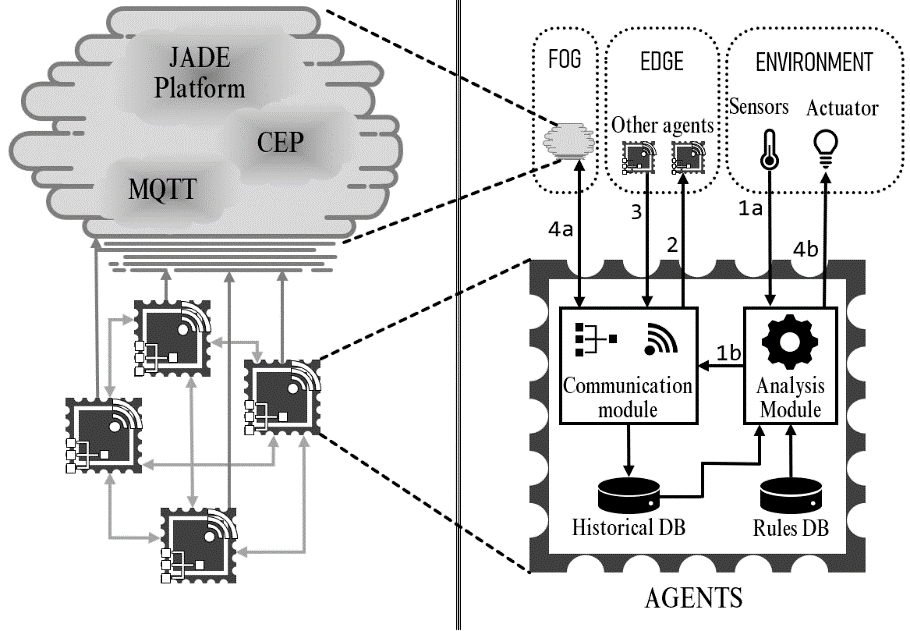
\includegraphics[scale=1.2]{chap1/archi2.png}
\caption{Edges nœuds et de leur communication avec le fog}
\label{archi22}
\end{figure}

\subsection{Perspicacité et Communications sur les edge nœuds}
Dans les edge nœuds, nous allons avoir, d'une part, la plate-forme JADE qui prend en charge les agents répartis entre les edge nœuds; et d'autre part, un moteur CEP. Puisque tous les messages reçus dans le fog sont formatés dans notre propre architecture, ils seront déjà dans un format homogène, ainsi nous éviterons le besoin d'un SOA 2.0 et d'un ESB et n'aurons besoin que du moteur CEP. Nous aurons également un courtier de messages pour offrir des revenus et des topics de message de sortie au fog nœud. Les événements pertinents détectés par les edge nœuds seront envoyés à la rubrique d'entrée; dans ce même sujet, les événements d'intérêt envoyés à partir du cloud ou d'autres fog nœuds seront reçus. Toutes les données reçues dans cette rubrique seront traitées par le moteur CEP qui téléchargera les nouvelles situations d'intérêt détectées dans le cloud, d'autres edge et fog nœuds , comme programmé dans le modèle via une nouvelle rubrique de sortie. De plus, l'utilisateur peut envoyer de nouvelles conditions aux edge nœuds via une rubrique et recevoir des informations d'intérêt par les mêmes moyens. Par conséquent, les communications de l’edge nœud, la passerelle.


Ainsi, le comportement est le suivant:
\begin{enumerate}
    \item Le fog nœud recevra les informations suivantes:
    \begin{itemize}
        \item Le fog nœud recevra les informations pertinentes soumises par les agents en edge via un topic de message.
 \item  En outre, le fog nœud recevra des informations pertinentes à traiter à partir du cloud. Ces informations seront reçues via le même topic de message.
 \item  Enfin, le fog nœud peut recevoir des informations pertinentes à traiter à partir d'autres fog nœuds , qui seront également reçues via le topic du message.

    \end{itemize}
    \item Lorsque les informations parviennent au Broker , elles sont envoyées au moteur CEP.
    \item Les informations étant traitées en temps réel dans le moteur CEP, diverses situations d'intérêt peuvent être détectées. Ces situations d'intérêt peuvent être envoyées à trois sorties.
    \begin{itemize}
        \item Situation pertinente d'intérêt pour les edge nœuds.
        \item Situation pertinente d'intérêt pour les nœuds cloud.
        \item Situation pertinente intéressant les autres fog nœuds.
    \end{itemize}
    \item Enfin, il y aura une communication directe avec l'utilisateur, qui ne passe pas par le moteur CEP:
    \begin{itemize}
        \item Les agents de l'edge soumettront les informations pertinentes à l'utilisateur, selon les règles programmées en eux; ces informations sont soumises via un topic de message.
\item L'utilisateur sera abonné à ce topic et recevra donc ces informations par son intermédiaire.
\item De même, l'utilisateur soumettra de nouvelles conditions, règles ou actions à l'edge via le topic du message.
\item Et les edges nœuds recevront ces informations via leur abonnement au topic.

    \end{itemize}
\end{enumerate}

\section{Modèle de coopération utilisé}
Nous avons mis en œuvre notre architecture pour créer un périphérique de sécurité IoT. Ceci, enfin, contrôle la sécurité d'un environnement contre les événements accidentels et accidentels. Son but est d'agir sur l'existence d'un criminel dans l'environnement. Et il peut contrôler les risques d'accident tels que les incendies et les fuites de gaz. La mise en œuvre est illustrée à la figure \ref{fc16} et expliquée ci-dessous.


Nous mettons en œuvre notre architecture proposée avec la carte Raspberry pi 2 (voir la partie gauche de la figure \ref{fc16}). Cette carte nous a permis de combiner les trois couches suivantes en une seule et même structure (comme illustré à droite de la figure  \ref{fc16}):
\begin{figure}[H]
\centering
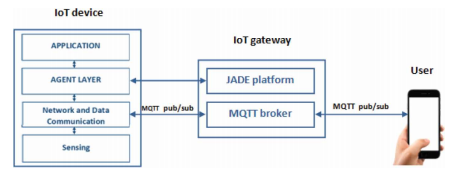
\includegraphics[scale=1.2]{chap1/fc16.png}
\caption{Architecture proposée pour le fonctionnement global}
\label{fc16}
\end{figure}


\textbf{La couche d'application (The Application Layer):} c'est une application d'un environnement de sécurité réel (maison, appartement, lieu de travail);


\textbf{La couche d'agent (The Agent Layer):} il s’agit d’un agent intégré dans l’instrument IoT, il gère les informations reçues par les capteurs, les analyse et prend des décisions.


\textbf{Couche de communication réseau et données (Network and Data Communication Layer):} le périphérique IoT communique avec les autres périphériques via cette couche;


\textbf{Couche de détection (Sensing Layer):} elle a été mise en œuvre sur le capteur de présence et le capteur d'humidité et de température.

\subsection{Communication entre les objets}

Afin de visualiser la communication inter objets , nous avons utiliser deux diagrammes de séquence de deux scénarios.

\subsubsection{Scénario de détection des voisinages:} pour un système dynamique et flexible, il est possible d'ajouter de nouveaux objets sans aucun problème. La figure \ref{fc17} illustre un diagramme de séquence décrivant comment les objets détectent leurs voisins. 

Dans le diagramme, l'objet du climatiseur diffuse le message "bonjour" au démarrage à tous les objets de l'environnement. Chaque objet reçoit le message, enregistre les informations du climatiseur en tant que nouvel objet et répond avec un autre message contenant son information. Avec cette méthode, le système a découvert les nouveaux objets de l'environnement.




\begin{figure}[H]
\centering
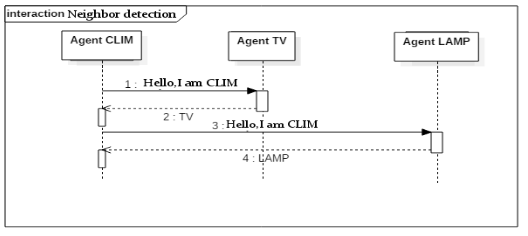
\includegraphics[scale=1.2]{chap1/fc17.png}
\caption{Diagramme de séquence de détection des voisins}
\label{fc17}
\end{figure}
\subsubsection{Scénario de détection de défaut:} pour créer un système complètement autonome et éviter le problème de la centralisation. Car dans ce cas , Si le composant central tombe en panne , tout le systeme y tombe en panne , pour cela On a proposé un systeme decentralisé et les objets échangent les informations entre eux et le système détecte les défaillances.


Chaque objet stocke des informations provenant d'objets voisins. Les objets diffusent toutes les 30 secondes leur état et enregistrent à l'aide de leurs voisins. Si un objet dépasse le délai de 30 secondes sans l'état de diffusion et que l'objet ne déclare pas que le système est éteint, il est considéré comme un échec.


Le système pris en charge demande au serveur de dépannage de réparer celui qui a échoué ou a appelé l’agence de dépannage pour réparer dans ce cas. Dans l'environnement, qui est responsable de l'information du serveur? Le système est centralisé n'est pas un composant responsable pour informer le serveur.


Résoudre ce problème en important la technique CSMA / CD \cite{6} utilisée dans les réseaux pour éviter les collisions. Dans notre cas, l’utilise pour sélectionner un objet qui joue le rôle d’informer le serveur de dépannage.

\begin{figure}[H]
\centering
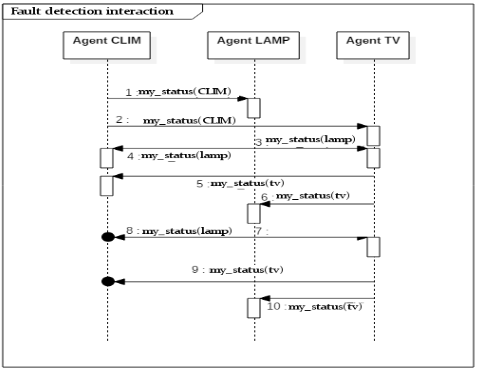
\includegraphics[scale=0.9]{chap1/fc18.png}
\caption{diagramme de séquence de détection des désactive et échoue}
\label{fc18}
\end{figure}

La technique est utilisée après la détection de l'échec. Chaque objet de notre système choisit un entier aléatoire et diffus ce nombre à tous les objets système. L'objet qui a le nombre maximum prend le rôle d'informer le serveur de dépannage.
\section{Conclusion}


Dans ce chapitre nous avons presenté nos contributions, nous avons commencé par l'architecture génerale de notre approche cloud computing baseé IoT pour le smart house, nous avons detaillé chaque éléments de l'architecture.

Nous avons detaillé les differents couches du dispositif IoT en ce concentrent sur la couche ajoutée qui est "Layer Agent",
Afin de minimiser le nombre de capteurs dans l'environement, nous avons montré l'IoT Robot que nous avons expliqué chaque module et le detaillé avec des diagrames.

Nous avons mis le point sur l'API que nous avons bati, cette API qui refléte un simulater de de maison intelligante.


En fin et afin de visualiser la communication inter objets ,nous utiliser deux diagrammes de sequence de deux scenaries.





